\section{Безопасность в статистических БД}

Инфы про статистические базы данных на русском языке мало и большая часть бредовая. Гуглите statistical database. Все источники будут на английском, переведено специально для вас. Источников несколько \cite{ComputerSecurity2008} \cite{IntroBD2014}, под конец была найдена статья, \cite{SDB1989} в которой есть вся собранная инфа, еще есть более свежий источник \citep{SDB1999}.

\subsection{Общие сведения}
Определение статистической БД. Классификация статистических БД. Характеристики статистических БД.

\paragraph{Определение статистической БД}
Статистической (в приведенном здесь контексте) называется база данных, в которой допускаются запросы с обобщением данных (суммированием, вычислением среднего значения и т.д.), но не допускаются запросы по отношению к элементарным данным. Например, в статистической базе данных разрешается выдача запроса "Какова средняя зарплата программистов?", тогда как выдача запроса "Какова зарплата программиста Мэри?" запрещена. Например, в СУБД PostreSQL есть набор агрегирующих запросов для получения статистических данных.
Угрозой безопасности статистических баз данных является то, что с помощью логических заключений на основе результатов выполнения разрешенных запросов можно вывести ответ, который прямо может быть получен только с помощью запрещенного запроса. "Обобщенные значения содержат следы исходной информации, и она может быть восстановлена злоумышленником после соответствующей обработки этих обобщенных значений. Такой процесс называется логическим выводом конфиденциальной информации".
Практически для любой статистической базы данных может быть определен общий трекер (в отличие от множества индивидуальных трекеров). Общий трекер (general tracker) — это логическое выражение, которое может быть использовано для поиска ответа на любой запрещенный запрос, т.е. запрос, включающий недопустимое логическое выражение. (В противоположность этому индивидуальный трекер работает только на основе запросов, включающих конкретные запрещенные выражения)
Таким образом, для обеспечения безопасности конфиденциальных данных в статистической БД требуется поддерживать баланс между репрезентативностью хранимой информации и конфиденциальностью отдельных записей.

\paragraph{Классификация статистических БД}
Классифицирует по следующим признакам:
\begin{itemize}

    \item Чисто статистическая база данных - обычная база данных со статистическим доступом

Чисто статистическая база данных хранит только уже обработанные статистические данные. Примером может служить база данных переписи населения.
Обычная БД содержит отдельные записи. Кроме того, обычная база данных поддерживает набор статистических пользователей, которым разрешены только статистические запросы. Для этих пользователей совокупная статистика, основанная на базовых необработанных данных, генерируется в ответ на запрос пользователя или может быть предварительно вычислена и сохранена как часть базы данных.

    \item Оффлайн-Онлайн

В онлайн-SDB (Statistical DataBase) существует прямое взаимодействие пользователя с данными в режиме реального времени через терминал. В автономной SDB пользователь не контролирует обработку данных и не знает, когда выполняется его запрос данных. В этом режиме методы защиты, отслеживающие поведение профилей пользователей, становятся более громоздкими. Методы компрометации, требующие большого количества запросов, также усложняются при работе в автономном режиме.

    \item Статическая-Динамическая

Статическая база данных~--- это такая база данных, которая никогда не меняется после ее создания. Большинство баз данных переписи являются статическими. Всякий раз, когда создается новая версия базы данных, эта новая версия считается другой статической базой данных (в отличие от динамических баз дынных, которые могут изменяться непрерывно). Эта особенность может значительно усложнить проблему защиты статической БД, поскольку частые выпуски новых версий могут позволить злоумышленнику использовать различия между версиями различными способами, которые трудно предвидеть. Методы защиты путем возмущения данных (см. далее) могут не подходить для динамических СДБ, так как усилия по преобразованию исходного СДБ в возмущенный в режиме реального времени могут стать непомерными.

    \item Централизованная-Децентрализованная

В централизованной SDB есть один объект базы данных. В децентрализованной (распределенной) SDB перекрывающиеся подмножества базы данных хранятся на различных узлах, соединенных коммуникационной сетью. Распределенная база данных может содержать полностью дублированные данные, частично дублированные или полностью разделенные. Проблема безопасности распределенной SDB является более сложной, чем проблема централизованной SDB из-за необходимости дублировать на каждом узле накладные расходы по контролю безопасности, а также из-за трудностей по отслеживанию и контролю профилей пользователей.

	\item Выделенная-общая компьютерная система

В выделенной для SDB компьютерной системе обслуживаются исключительно приложения для работы с SDB. В общей системе приложения SDB работают на одной аппаратной платформе с другими приложениями (возможно, использующие различные базы данных). Общую среду защитить сложнее, так как другие приложения могут вмешиваться в защищаемые данные непосредственно через операционную систему, минуя механизм безопасности SDB.
\end{itemize}
\subsection{Угрозы статистических БД}

О безопасности в статистических БД  Деннинг [16.6]
\begin{grayquote}
"Методы нарушения защиты данных просты и не связаны с большими расходами. Поэтому требование обеспечения полной секретности конфиденциальной информации несовместимо с требованием возможности вычисления точных статистических показателей для произвольных подмножеств данных в базе. По крайней мере одно из этих требований должно быть снято прежде, чем можно будет поверить в гарантии обеспечения секретности."
\end{grayquote}
Таким образом, существует мнение, что нельзя нормально обезопасить СБД.

Основная уязвимость для несанкционированного доступа к данным в СБД -- проблема вывода.
В общих чертах, проблема вывода для SDB может быть сформулирована следующим образом. Характеристическая функция C определяет подмножество записей (строк) в базе данных. Запрос, использующий C, предоставляет статистику по выбранному подмножеству. Если подмножество достаточно мало, возможно, даже одна запись, спрашивающий может быть в состоянии сделать вывод о характеристиках одного человека или небольшой группы. Даже для больших подмножеств характер или структура данных могут быть такими, что информация, доступа к которой быть не должно, может быть получена злоумышленником.
Для злоумышленика, который пытается достать индивидуальные данные, задача состоит в том, чтобы сделать общий трекер.
Нужно придумать такую последовательность запросов, чтобы вывести индививидуальную информацию.

Например, для статичной СБД можно реализовать подобную атаку:

Запрос1: выдать a1 + a2 + a3. Запрос2: выдать a1 + a2. Запрос1 - Запрос2 = a3.

Для динамической онлайн СБД атака может иметь подобную модель:
Злоумышленник хочет узнать зарплату Мэри. Он знает, что ей 20 лет. Он записываем в базу много "пустых" записей с возрастом = 20 лет и нулевой зарплатой. Злоумышленник делает запрос с минимальной агрегацией людей с возврастом 20 лет. Таким образом можно узнать возможную зарплату Мэри. Чем больше исходных знаний есть о Мэри, тем точнее получатся данные.
Также не стоит забывать что речь идет о БД. Поэтому статистическая БД наследует все угрозы обычных БД.

  \subsection{Защита в статистических БД}

Разделяют четыре общих подхода защиты статистических БД:
\begin{itemize}
  \item концептуальный;
	\item ограничение запросов;
	\item возмущение данных;
	\item возмущение вывода;
\end{itemize}
На рисунке \ref{fig:SDB_secure} изображена схема 3 подходов: ограничение запросов, возмущение данных, возмущение вывода.
\begin{figure}[h]
    \centering
    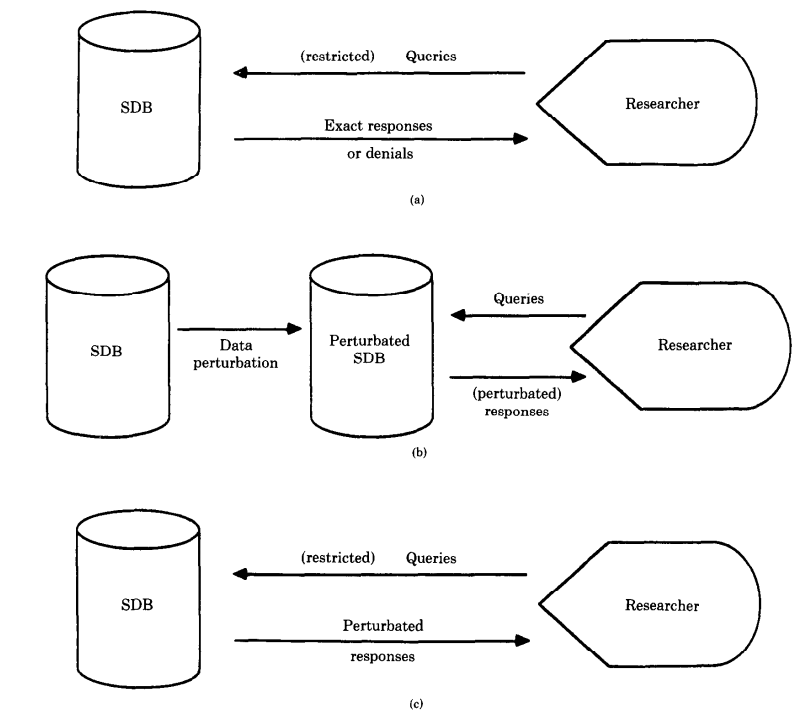
\includegraphics[width=0.8\textwidth]{assets/SDB_secure_method.png}
    \caption{Схемы безопасности СДБ}
    \label{fig:SDB_secure}
\end{figure}
\paragraph{Концептуальный}

Основная проблема защиты статистических БД в том, что вся реляционная алгебра, которую различным образом реализуют языки манипуляции данными, позволяет выводить индивидуальные данные. Концептуальный подход предлагает заменить классическую схему взаимодействия с данными реляционной БД. Для этого были описаны качественные требования к фреймворку (формальное доказательство требований имеется в статье \cite{LatticeModel}), реализующему новую логику взаимодействия:
\begin{enumerate}
  \item Необходимо учитывать категории данных в таблицах (например, категоризация людей по профессии)
  \item Необходимо принимать во внимание динамически изменяемые данные и угрозы, связанные с этим
  \item Необходимо учитывать знания, полученныые каждым пользователем после запросов
  \item Необходимо учитывать возможный вывод информации (в общем случае или с учетом знаний пользователя)
\end{enumerate}

Для выполнения требований в основном используется создание единицы неразложимой подгруппы данных (subpopulation). В таких объектах содержаться 0 или больше двух реальных записей. Определение такой подгруппы контролируется DBA. В определении подгруппы содержится информация о разрешенных типах статистических запросов для каждого атрибута и ограничения, связанные с обновлением данных. В ядре фреймворка есть процесс, отслеживающий знания группы пользователей, полученные из предыдущих запросов. Также используется процесс отслеживания знаний пользователя при динамических операциях с данными в БД. Все процессы имеют связь с помощью сообщений с DBA.

Еще один способ концептуального подхода -- использование решетчетой модели, который заключается в агрегации данных по разным признакам на разном уровне детализации (то есть выделение отдельных таблиц с меньшим количеством атрибутов и с одним или более одинаковыми признаками (берем общее поле, например пол, и все записи одникового пола переносим в отдельные таблицы)).

Классический способ (не защищающий от вывода данных) -- для пользователей с доступом к персональным данным доступны все запросы. А исследователям статистики и прочим пользователям без доступа к персональным данным выдается доступ только к некоторым записям или готовым статистическим результатам (агрегация).

Сама конциептуальная модель описана только в более старой статье \cite{SDB1989}, в новых статьях \cite{SDB1999}, \cite{ComputerSecurity2008} она уже не упоминается.

\paragraph{Ограничение запросов}

Для ограничения запросов используется 5 стандартных методов: ограничение размера выдаваемой выборки, контроль перекрытия результатов, аудит, подавление ячеек и разделение.

\begin{enumerate}

  \item Ограничение размера выборки

Это ограничение требует параметр K, который задается администратором БД. Размер C выдаваемой выборки удовлетворяет условию (L - общее число записей):

\begin{displaymath}
K \leq C \leq L - K, \quad K < L/2
\end{displaymath}

  \item Контроль перекрытия запросов

Зачастую для вывода данных используется перекрытие запросов. Поэтому необходимо ограничить количество перекрывающихся записей. Однако на практике это не защищает от сотрудничества нескольких пользователей, ограничивая полезные функций БД и увеличивая сложность сравнения результатов запросов.

  \item Аудит

Метод заключается в сохранении запросов пользователя и анализе на возможность компрометации. Сложность, связанная с вычислительной нагрузкой, остается.

  \item Разделение

Основная идея разделения -- это перегруппировка на непересекающиеся множества, объединенные некоторым признаком, называемые атомарными множествами.

  \item Подавление ячеек

Подавление ячеек -- это сокрытие информации в ячейках, которые могут привести к раскрытию конфиденциальной информации. Кроме того, есть дополнительное подавление -- когда скрывают ячейки с неконфиденциальной информацией, которые могут косвенно использоваться для раскрытия конфиденциальной информации.

\end{enumerate}

Стоит отметить, что ни один из предложенных методов не дает универсальное решение.

\paragraph{Возмущение данных}

Методы возмущения данных делятся на две категории: категория распределения вероятностей и категория возмущения фиксированных данных. Первые из них рассматривают данные как распределение вероятностей и подменяют исходные данные на новые таблицы, сгенерированные на основе полученного распределения. Вторые вычисляют статистику фиксированных данных и на основе статистики раз и навсегда возмущают имеющиеся данные. Для возмущения данных требуется специально преобразованная для статистических исследований исходная база данных. Важно отметить, что при возмущении данных могут меняться условные средние значения и частоты, что является негативным последствием.

\begin{enumerate}
  \item Распределение вероятностей

Для этой категории существует два основных метода: использование исходной выборки и выборки, полученной из распределения вероятностей исходной, и замена исходной БД на ее распределение вероятностей.

  \item Возмущение фиксированных данных

Возмущение происходит только для числовых или категорезированных данных.

\end{enumerate}


Рассмотрим два конкретных метода возмущения данных.
Случайное добавление дополнительных строк к основному набору данных, обрабатываемому запросом.
Второй способ -- "обмен данными" ("data swapping"), т.е. обмен значениями атрибутов между кортежами, осуществляемый таким образом, чтобы поддерживалась лишь статистическая точность. При этом даже если злоумышленнику удастся идентифицировать отдельное значение (например, некоторое значение зарплаты), то у него не будет способа узнать, какому именно кортежу (в нашем примере — сотруднику) оно принадлежит. Сложность этого подхода заключается в необходимости отыскать множество тех записей, между которыми можно будет организовать обмен значениями соответствующим образом. Подобные затруднения имеют место и при использовании других методов.

\paragraph{Возмущение вывода}

Отмеченная проблема изменения статистически важных данных условных средних значений частот не так серьезна в этом случае, так как возмущение накладывается на уже выходные данные.

Для того, чтобы определить выходную выборку, каждая запись проходит через функцию, которая с некоторой ненулевой вероятностью помещает запись в выходную выборку. Эта вероятность может корректироваться администратором базы данных.

  \subsection{Критерии безопасности}

Как было сказано, гарантированной безопасности в СДБ не добиться. Поэтому оценивается степень деанонимизированности данных и статистического соответствия исходным данным.

Security~--- вероятность раскрыть (в том числе частично) запись в СБД. Для каждого разрешенного агрегирующего запроса оценивается критерий безопасности. На основе количества информации в базе можно подсчитать, сколько тех или иных запросов нужно сделать для деанонимизации. На основе этого расчитывается минимальная выборка для таких запросов.

Consistency -- оценивается консистентность данных для методов возмущения данных. Оценивается степень возмущения данных. Для этого создается агрегирующий запрос и замеряется его изменения после внесенных возмущений.

Robustness -- оценка зависимости между возмущением и конкретной записью. Необходимо, чтобы возмущение не было зависимо от данных, но при этом нужно сохранить ее статистические свойства.

Costs -- назначение каждому запросу конкретной цены. Пользователю дается начальная сумма, на которую он может делать запросы, такая, чтобы он не смог вывести данные.
